% Presentación final (E11) alineada a los criterios de §16 de la especificación v1.5.
% Compilar: python EntregaFinal/documentos/compilar.py presentacion   (12 a 15 diapositivas; arma también el .pptx)
% Estilo: el del tablero (dash_app/DISENO.md): página gris, tarjetas casi blancas, títulos grandes en peso normal,
% chips en píldora blanca y los colores por rol de generado/colores.tex. Las notas del orador están en notas_orador.txt.
\documentclass[aspectratio=169,10pt]{beamer}
\usepackage{fontspec}
% Sin alternativas contextuales (calt): el texto del PDF se copia y se extrae completo (guiones, dos puntos y
% paréntesis), lo que también permite armar el .pptx con texto editable.
\defaultfontfeatures{RawFeature={-calt}}
\setsansfont{Inter-Regular.ttf}[Path=fuentes/, BoldFont=Inter-SemiBold.ttf, ItalicFont=Inter-Regular.ttf,
  ItalicFeatures={FakeSlant=0.16}]
\setmonofont{Inter-Regular.ttf}[Path=fuentes/]
\newfontfamily\intermedia{Inter-Medium.ttf}[Path=fuentes/]
\usepackage[spanish,es-noshorthands,es-tabla]{babel}
% Generado por documentos/datos_documentos.py desde dash_app/tokens.py (roles de DISENO.md §2).
\definecolor{rol-real}{RGB}{20,20,20}
\definecolor{rol-hoy}{RGB}{133,133,133}
\definecolor{rol-contexto}{RGB}{200,200,200}
\definecolor{rol-modelo}{RGB}{36,87,240}
\definecolor{rol-modelo-final}{RGB}{36,87,240}
\definecolor{rol-previsto-modelo}{RGB}{36,87,240}
\definecolor{rol-previsto-hoy}{RGB}{133,133,133}
\definecolor{rol-recorta}{RGB}{184,35,95}
\definecolor{rol-oraculo}{RGB}{20,20,20}
\definecolor{rol-modelo-tinte}{RGB}{220,229,253}
\definecolor{rol-hoy-tinte}{RGB}{227,227,227}
\definecolor{rol-recorta-tinte}{RGB}{246,219,230}
\definecolor{rol-referencia}{RGB}{102,102,102}
\definecolor{rol-cero}{RGB}{102,102,102}
\definecolor{rol-rejilla}{RGB}{235,235,235}
\definecolor{rol-eje}{RGB}{208,208,208}
\definecolor{rol-silencio}{RGB}{13,148,136}
\definecolor{rol-cra54}{RGB}{232,89,12}
\definecolor{rol-cl72}{RGB}{112,72,232}
\definecolor{rol-bien}{RGB}{24,117,58}
\definecolor{rol-atencion}{RGB}{178,111,11}
\definecolor{rol-atencion-texto}{RGB}{146,91,8}
\definecolor{rol-critico}{RGB}{186,43,46}
\definecolor{rol-acento}{RGB}{36,87,240}
\definecolor{rol-acento-fuerte}{RGB}{27,68,200}
\definecolor{rol-acento-suave}{RGB}{228,235,254}
\definecolor{rol-foco}{RGB}{36,87,240}
\definecolor{rol-tinta}{RGB}{20,20,20}
\definecolor{rol-tinta-2}{RGB}{85,85,85}
\definecolor{rol-tinta-3}{RGB}{102,102,102}
\definecolor{rol-tinta-tenue}{RGB}{138,138,138}
\definecolor{rol-tinta-inversa}{RGB}{255,255,255}
\definecolor{rol-blanco}{RGB}{255,255,255}
\definecolor{rol-superficie}{RGB}{250,250,250}
\definecolor{rol-superficie-2}{RGB}{233,233,233}
\definecolor{rol-fondo}{RGB}{239,239,239}
\definecolor{rol-linea}{RGB}{227,227,227}
\definecolor{rol-linea-fuerte}{RGB}{208,208,208}
\definecolor{rol-pantalla-inicio}{RGB}{20,20,20}
\definecolor{rol-pantalla-pronostico}{RGB}{20,20,20}
\definecolor{rol-pantalla-horario}{RGB}{20,20,20}
\definecolor{rol-pantalla-modelo}{RGB}{20,20,20}
\definecolor{rol-pantalla-resultado}{RGB}{20,20,20}
\definecolor{rol-pantalla-enlaces}{RGB}{20,20,20}

% Generado por documentos/datos_documentos.py: no editar a mano. Cada cifra con su evidencia.

\newcommand{\ModeloActivo}{hgb\_fv2\_20250831\_s42}% api_frecuencias/docs/evidencias/modelo/evaluacion_modelo.json
\newcommand{\PruebaDesde}{2025-11-01}% api_frecuencias/docs/evidencias/modelo/evaluacion_modelo.json
\newcommand{\PruebaHasta}{2025-12-31}% api_frecuencias/docs/evidencias/modelo/evaluacion_modelo.json
\newcommand{\Nprueba}{3.111}% api_frecuencias/docs/evidencias/modelo/evaluacion_modelo.json
\newcommand{\WAPEact}{14,77}% api_frecuencias/docs/evidencias/modelo/evaluacion_modelo.json
\newcommand{\MAEact}{96,27}% api_frecuencias/docs/evidencias/modelo/evaluacion_modelo.json
\newcommand{\WAPEactIC}{13,10--16,87}% api_frecuencias/docs/evidencias/modelo/evaluacion_modelo.json
\newcommand{\WAPEfvuno}{15,07}% api_frecuencias/docs/evidencias/modelo/evaluacion_modelo.json
\newcommand{\MAEfvuno}{98,20}% api_frecuencias/docs/evidencias/modelo/evaluacion_modelo.json
\newcommand{\WAPEfvunoIC}{13,22--17,43}% api_frecuencias/docs/evidencias/modelo/evaluacion_modelo.json
\newcommand{\WAPEbuno}{21,18}% api_frecuencias/docs/evidencias/modelo/evaluacion_modelo.json
\newcommand{\MAEbuno}{138,06}% api_frecuencias/docs/evidencias/modelo/evaluacion_modelo.json
\newcommand{\WAPEbunoIC}{16,61--26,79}% api_frecuencias/docs/evidencias/modelo/evaluacion_modelo.json
\newcommand{\WAPEbdos}{26,40}% api_frecuencias/docs/evidencias/modelo/evaluacion_modelo.json
\newcommand{\MAEbdos}{172,05}% api_frecuencias/docs/evidencias/modelo/evaluacion_modelo.json
\newcommand{\WAPEbdosIC}{22,77--30,57}% api_frecuencias/docs/evidencias/modelo/evaluacion_modelo.json
\newcommand{\SesgoAct}{2,75}% api_frecuencias/docs/evidencias/modelo/evaluacion_modelo.json
\newcommand{\DifActBunoIC}{−10,43 a −3,21}% api_frecuencias/docs/evidencias/modelo/evaluacion_modelo.json
\newcommand{\PmejoraActBuno}{1,00}% api_frecuencias/docs/evidencias/modelo/evaluacion_modelo.json
\newcommand{\MejoraRelBuno}{30}% api_frecuencias/docs/evidencias/modelo/evaluacion_modelo.json
\newcommand{\CobModelo}{79,49}% api_frecuencias/docs/evidencias/modelo/evaluacion_modelo.json
\newcommand{\CobConformal}{77,88}% api_frecuencias/docs/evidencias/modelo/evaluacion_modelo.json
\newcommand{\BajoPdiez}{13,28}% api_frecuencias/docs/evidencias/modelo/evaluacion_modelo.json
\newcommand{\SobrePnoventa}{8,84}% api_frecuencias/docs/evidencias/modelo/evaluacion_modelo.json
\newcommand{\WAPEPico}{14,38}% api_frecuencias/docs/evidencias/modelo/evaluacion_modelo.json
\newcommand{\WAPEValle}{14,97}% api_frecuencias/docs/evidencias/modelo/evaluacion_modelo.json
\newcommand{\WAPERutaSilencio}{15,33}% api_frecuencias/docs/evidencias/modelo/evaluacion_modelo.json
\newcommand{\WAPERutaSilencioBuno}{21,30}% api_frecuencias/docs/evidencias/modelo/evaluacion_modelo.json
\newcommand{\WAPERutaCra}{13,04}% api_frecuencias/docs/evidencias/modelo/evaluacion_modelo.json
\newcommand{\WAPERutaCraBuno}{19,79}% api_frecuencias/docs/evidencias/modelo/evaluacion_modelo.json
\newcommand{\WAPERutaCl}{19,23}% api_frecuencias/docs/evidencias/modelo/evaluacion_modelo.json
\newcommand{\WAPERutaClBuno}{25,27}% api_frecuencias/docs/evidencias/modelo/evaluacion_modelo.json
\newcommand{\RobDosmilveinticuatro}{16,26}% api_frecuencias/docs/evidencias/modelo/evaluacion_modelo.json
\newcommand{\RobDosmilveinticuatroIC}{14,97--17,91}% api_frecuencias/docs/evidencias/modelo/evaluacion_modelo.json
\newcommand{\RobDosmilveinticuatroBuno}{21,55}% api_frecuencias/docs/evidencias/modelo/evaluacion_modelo.json
\newcommand{\RobDosmilveinticinco}{14,48}% api_frecuencias/docs/evidencias/modelo/evaluacion_modelo.json
\newcommand{\RobDosmilveinticincoIC}{13,78--15,28}% api_frecuencias/docs/evidencias/modelo/evaluacion_modelo.json
\newcommand{\RobDosmilveinticincoBuno}{20,04}% api_frecuencias/docs/evidencias/modelo/evaluacion_modelo.json
\newcommand{\CobVdos}{77,82}% api_frecuencias/docs/evidencias/modelo/calibracion_condicional.json
\newcommand{\BajoPdiezVdos}{12,95}% api_frecuencias/docs/evidencias/modelo/calibracion_condicional.json
\newcommand{\SobrePnoventaVdos}{9,23}% api_frecuencias/docs/evidencias/modelo/calibracion_condicional.json
\newcommand{\AnchoVdos}{303,4}% api_frecuencias/docs/evidencias/modelo/calibracion_condicional.json
\newcommand{\CobVuno}{77,88}% api_frecuencias/docs/evidencias/modelo/calibracion_condicional.json
\newcommand{\BajoPdiezVuno}{13,28}% api_frecuencias/docs/evidencias/modelo/calibracion_condicional.json
\newcommand{\SobrePnoventaVuno}{8,84}% api_frecuencias/docs/evidencias/modelo/calibracion_condicional.json
\newcommand{\AnchoVuno}{312,9}% api_frecuencias/docs/evidencias/modelo/calibracion_condicional.json
\newcommand{\CalibPeorDesv}{4,15}% api_frecuencias/docs/evidencias/modelo/calibracion_condicional.json
\newcommand{\HorTreinta}{19,43}% api_frecuencias/docs/evidencias/modelo/horizontes.json
\newcommand{\HorTreintaBuno}{23,12}% api_frecuencias/docs/evidencias/modelo/horizontes.json
\newcommand{\HorSesenta}{14,71}% api_frecuencias/docs/evidencias/modelo/horizontes.json
\newcommand{\HorSesentaBuno}{18,96}% api_frecuencias/docs/evidencias/modelo/horizontes.json
\newcommand{\HorCientoveinte}{10,87}% api_frecuencias/docs/evidencias/modelo/horizontes.json
\newcommand{\HorCientoveinteBuno}{15,44}% api_frecuencias/docs/evidencias/modelo/horizontes.json
\newcommand{\HorEvaluado}{2025-03-01 a 2025-12-31}% api_frecuencias/docs/evidencias/modelo/horizontes.json
\newcommand{\AlertasAhora}{0,53}% api_frecuencias/docs/evidencias/alertas/backtest_alertas.json
\newcommand{\AlertasAntes}{6,08}% api_frecuencias/docs/evidencias/alertas/backtest_alertas.json
\newcommand{\AlertasObsTodas}{1,24}% api_frecuencias/docs/evidencias/alertas/backtest_alertas.json
\newcommand{\DiasRuta}{324}% api_frecuencias/docs/evidencias/alertas/backtest_alertas.json
\newcommand{\AlertasDesde}{2025-09-15}% api_frecuencias/docs/evidencias/alertas/backtest_alertas.json
\newcommand{\AlertasHasta}{2025-12-31}% api_frecuencias/docs/evidencias/alertas/backtest_alertas.json
\newcommand{\LiftCinco}{4,69}% api_frecuencias/docs/evidencias/alertas/backtest_alertas.json
\newcommand{\LiftAntesCinco}{1,77}% api_frecuencias/docs/evidencias/alertas/backtest_alertas.json
\newcommand{\PrecCinco}{0,36}% api_frecuencias/docs/evidencias/alertas/backtest_alertas.json
\newcommand{\LiftSeis}{8,30}% api_frecuencias/docs/evidencias/alertas/backtest_alertas.json
\newcommand{\LiftAntesSeis}{1,31}% api_frecuencias/docs/evidencias/alertas/backtest_alertas.json
\newcommand{\PrecSeis}{0,39}% api_frecuencias/docs/evidencias/alertas/backtest_alertas.json
\newcommand{\LiftSiete}{1,34}% api_frecuencias/docs/evidencias/alertas/backtest_alertas.json
\newcommand{\LiftAntesSiete}{0,78}% api_frecuencias/docs/evidencias/alertas/backtest_alertas.json
\newcommand{\PrecSiete}{0,27}% api_frecuencias/docs/evidencias/alertas/backtest_alertas.json
\newcommand{\LiftOcho}{3,78}% api_frecuencias/docs/evidencias/alertas/backtest_alertas.json
\newcommand{\LiftAntesOcho}{2,87}% api_frecuencias/docs/evidencias/alertas/backtest_alertas.json
\newcommand{\PrecOcho}{0,70}% api_frecuencias/docs/evidencias/alertas/backtest_alertas.json
\newcommand{\UOcupCritica}{0,90}% api_frecuencias/docs/evidencias/alertas/backtest_alertas.json
\newcommand{\UBajaUtil}{0,30}% api_frecuencias/docs/evidencias/alertas/backtest_alertas.json
\newcommand{\UCaida}{0,30}% api_frecuencias/docs/evidencias/alertas/backtest_alertas.json
\newcommand{\UPersistencia}{2}% api_frecuencias/docs/evidencias/alertas/backtest_alertas.json
\newcommand{\UErrorPron}{0,15}% api_frecuencias/docs/evidencias/alertas/backtest_alertas.json
\newcommand{\UZ}{3,5}% api_frecuencias/docs/evidencias/alertas/backtest_alertas.json
\newcommand{\UTolDespacho}{5}% api_frecuencias/docs/evidencias/alertas/backtest_alertas.json
\newcommand{\UTolSalidas}{0,50}% api_frecuencias/docs/evidencias/alertas/backtest_alertas.json
\newcommand{\UAtraso}{2}% api_frecuencias/docs/evidencias/alertas/backtest_alertas.json
\newcommand{\UWapeMax}{0,20}% api_frecuencias/docs/evidencias/alertas/backtest_alertas.json
\newcommand{\USemanasRef}{8}% api_frecuencias/docs/evidencias/alertas/backtest_alertas.json
\newcommand{\UTolSalidasPct}{50}% api_frecuencias/docs/evidencias/alertas/backtest_alertas.json
\newcommand{\UUnoMenosCaida}{0,70}% api_frecuencias/docs/evidencias/alertas/backtest_alertas.json
\newcommand{\AlertasAhoraDosmil}{0,45}% api_frecuencias/docs/evidencias/alertas/backtest_alertas_corte_2024-12-31.json
\newcommand{\AlertasAntesDosmil}{5,70}% api_frecuencias/docs/evidencias/alertas/backtest_alertas_corte_2024-12-31.json
\newcommand{\AlertasPronUno}{0,44}% api_frecuencias/docs/evidencias/alertas/backtest_alertas_pronostico.json
\newcommand{\AlertasPronDos}{0,32}% api_frecuencias/docs/evidencias/alertas/backtest_alertas_pronostico.json
\newcommand{\AlertasPronTres}{0,38}% api_frecuencias/docs/evidencias/alertas/backtest_alertas_pronostico.json
\newcommand{\AlertasPronCuatro}{0,03}% api_frecuencias/docs/evidencias/alertas/backtest_alertas_pronostico.json
\newcommand{\AlertasPronostico}{1,16}% api_frecuencias/docs/evidencias/alertas/backtest_alertas_pronostico.json
\newcommand{\AlertasTotal}{2,40}% api_frecuencias/docs/evidencias/alertas/backtest_alertas_pronostico.json
\newcommand{\ViablesBacktest}{46,0}% api_frecuencias/docs/evidencias/alertas/backtest_alertas_pronostico.json
\newcommand{\RevisionDoble}{dos revisores automatizados con un protocolo escrito, conciliación y kappa de Cohen de 0,80}% api_frecuencias/docs/evidencias/alertas/revision_doble/conciliacion.json
\newcommand{\Kpnoventaycinco}{451}% api_frecuencias/docs/evidencias/pruebas/k6_consultas.json
\newcommand{\Kpnoventaynueve}{572}% api_frecuencias/docs/evidencias/pruebas/k6_consultas.json
\newcommand{\Kpeticiones}{3.553}% api_frecuencias/docs/evidencias/pruebas/k6_consultas.json
\newcommand{\Ktasa}{58,8}% api_frecuencias/docs/evidencias/pruebas/k6_consultas.json
\newcommand{\Kerrores}{0,00}% api_frecuencias/docs/evidencias/pruebas/k6_consultas.json
\newcommand{\Kvus}{50}% api_frecuencias/docs/evidencias/pruebas/k6_consultas.json
\newcommand{\Kingesta}{722}% api_frecuencias/docs/evidencias/pruebas/k6_ingesta.json
\newcommand{\IngestaFilas}{111.792}% api_frecuencias/docs/evidencias/rendimiento.txt
\newcommand{\IngestaSegundos}{4,07}% api_frecuencias/docs/evidencias/rendimiento.txt
\newcommand{\IngestaTasa}{27.469}% api_frecuencias/docs/evidencias/rendimiento.txt
\newcommand{\IngestaMemoria}{53}% api_frecuencias/docs/evidencias/rendimiento.txt
\newcommand{\Ntotal}{1.060}% api_frecuencias/docs/evidencias/pruebas/suite_final.xml
\newcommand{\Npasan}{1.055}% api_frecuencias/docs/evidencias/pruebas/suite_final.xml
\newcommand{\Nfallan}{0}% api_frecuencias/docs/evidencias/pruebas/suite_final.xml
\newcommand{\Nomitidas}{5}% api_frecuencias/docs/evidencias/pruebas/suite_final.xml
\newcommand{\NUnit}{567}% api_frecuencias/docs/evidencias/pruebas/suite_final.xml
\newcommand{\NInteg}{106}% api_frecuencias/docs/evidencias/pruebas/suite_final.xml
\newcommand{\NReplica}{185}% api_frecuencias/docs/evidencias/pruebas/suite_final.xml
\newcommand{\NContrato}{178}% api_frecuencias/docs/evidencias/pruebas/suite_final.xml
\newcommand{\NDatos}{24}% api_frecuencias/docs/evidencias/pruebas/suite_final.xml
\newcommand{\NTcont}{8}% api_frecuencias/docs/evidencias/pruebas/ci/pytest.xml
\newcommand{\NTcontNota}{ (en su trabajo del CI)}% api_frecuencias/docs/evidencias/pruebas/ci/pytest.xml
\newcommand{\FechaPruebas}{2026-11-09 12:37}% api_frecuencias/docs/evidencias/pruebas/suite_final.xml
\newcommand{\CorridaPruebas}{corrida final de la suite completa (2026-11-09 12:37)}% api_frecuencias/docs/evidencias/pruebas/suite_final.xml
\newcommand{\Cobertura}{94,3}% api_frecuencias/docs/evidencias/pruebas/coverage_final.xml
\newcommand{\NIntentosLector}{32}% api_frecuencias/docs/evidencias/pruebas/suite_final.xml
\newcommand{\NIntentosEscritor}{84}% api_frecuencias/docs/evidencias/pruebas/suite_final.xml
\newcommand{\NIntentosTotal}{116}% api_frecuencias/docs/evidencias/pruebas/suite_final.xml
\newcommand{\FuenteIntentos}{\path{api_frecuencias/docs/evidencias/pruebas/suite_final.xml}}% api_frecuencias/docs/evidencias/pruebas/suite_final.xml
\newcommand{\EstadoCI}{en verde en GitHub Actions (run 42627652053, 2026-11-09)}% api_frecuencias/docs/evidencias/pruebas/ci_github.txt
\newcommand{\EstadoCICorto}{en verde en GitHub Actions (run 42627652053, 2026-11-09)}% api_frecuencias/docs/evidencias/pruebas/ci_github.txt
\newcommand{\GateCandidato}{hgb\_fv1\_20250831\_s42}% api_frecuencias/docs/evidencias/monitoreo/compuerta_ejemplo.json
\newcommand{\GateWAPECand}{12,97}% api_frecuencias/docs/evidencias/monitoreo/compuerta_ejemplo.json
\newcommand{\GateWAPEAct}{13,02}% api_frecuencias/docs/evidencias/monitoreo/compuerta_ejemplo.json
\newcommand{\GateDecision}{aprobado}% api_frecuencias/docs/evidencias/monitoreo/compuerta_ejemplo.json
\newcommand{\GateVentana}{2025-09-01 a 2025-09-14}% api_frecuencias/docs/evidencias/monitoreo/compuerta_ejemplo.json
\newcommand{\NVariables}{23}% api_frecuencias/docs/evidencias/monitoreo/onnx_paridad.json
\newcommand{\FeatureVersion}{fv2-2026-11-09}% api_frecuencias/docs/evidencias/monitoreo/onnx_paridad.json
\newcommand{\OnnxDifMax}{0,0028}% api_frecuencias/docs/evidencias/monitoreo/onnx_paridad.json
\newcommand{\OnnxMsFila}{0,10}% api_frecuencias/docs/evidencias/monitoreo/onnx_paridad.json
\newcommand{\SklearnMsFila}{12,6}% api_frecuencias/docs/evidencias/monitoreo/onnx_paridad.json
\newcommand{\FranjasTotal}{13}% api_frecuencias/docs/evidencias/optimizacion/sensibilidad.md
\newcommand{\FranjasViables}{11}% api_frecuencias/docs/evidencias/optimizacion/sensibilidad.md
\newcommand{\FranjasMilpIgual}{13}% api_frecuencias/docs/evidencias/optimizacion/sensibilidad.md
\newcommand{\FranjasNoViables}{CRA 54 (laboral, 7~h) y CRA 54 (sábado, 7~h)}% api_frecuencias/docs/evidencias/optimizacion/sensibilidad.md
\newcommand{\PlanRuta}{CRA 54}% api_frecuencias/docs/evidencias/optimizacion/ejemplo_plan_d5.json
\newcommand{\PlanFecha}{2025-11-19}% api_frecuencias/docs/evidencias/optimizacion/ejemplo_plan_d5.json
\newcommand{\PlanSalidas}{247}% api_frecuencias/docs/evidencias/optimizacion/ejemplo_plan_d5.json
\newcommand{\PlanProgramadas}{290,2}% api_frecuencias/docs/evidencias/optimizacion/ejemplo_plan_d5.json
\newcommand{\PlanHoraPico}{5}% api_frecuencias/docs/evidencias/optimizacion/ejemplo_plan_d5.json
\newcommand{\PlanHeadwayPico}{2,0}% api_frecuencias/docs/evidencias/optimizacion/ejemplo_plan_d5.json
\newcommand{\PlanSalidasPico}{30}% api_frecuencias/docs/evidencias/optimizacion/ejemplo_plan_d5.json
\newcommand{\PlanHeadwayMax}{8,5}% api_frecuencias/docs/evidencias/optimizacion/ejemplo_plan_d5.json
\newcommand{\SonarResumen}{SonarQube: puerta de calidad aprobada (vulnerabilidades: 0; errores: 0; bloqueantes: 0; críticos: 0; duplicación: 0,0~\%; cobertura: 94,3~\%)}% api_frecuencias/docs/evidencias/sonarqube/measures.json
\newcommand{\SonarCorto}{SonarQube: puerta de calidad aprobada (vulnerabilidades: 0; errores: 0; bloqueantes: 0; críticos: 0)}% api_frecuencias/docs/evidencias/sonarqube/measures.json
\newcommand{\SonarPuerta}{puerta de calidad aprobada}% api_frecuencias/docs/evidencias/sonarqube/measures.json
\newcommand{\SonarPruebas}{1.055}% api_frecuencias/docs/evidencias/sonarqube/measures.json
\newcommand{\DemoFilasInicial}{49.623}% api_frecuencias/docs/evidencias/despliegue/demo_ciclo_api.txt
\newcommand{\DemoFilasNuevas}{51}% api_frecuencias/docs/evidencias/despliegue/demo_ciclo_api.txt
\newcommand{\DemoFilasRepeticion}{0}% api_frecuencias/docs/evidencias/despliegue/demo_ciclo_api.txt
\newcommand{\DemoMarcaAntes}{2025-08-30}% api_frecuencias/docs/evidencias/despliegue/demo_ciclo_api.txt
\newcommand{\DemoMarcaDespues}{2025-08-31}% api_frecuencias/docs/evidencias/despliegue/demo_ciclo_api.txt
\newcommand{\DemoWapeNuevo}{26,5}% api_frecuencias/docs/evidencias/despliegue/demo_ciclo_api.txt
\newcommand{\DemoCandidato}{hgb\_fv2\_20250930\_s42}% api_frecuencias/docs/evidencias/despliegue/demo_ciclo_api.txt
\newcommand{\DemoEntrenoSeg}{37}% api_frecuencias/docs/evidencias/despliegue/demo_ciclo_api.txt
\newcommand{\DemoWapeCand}{14,11}% api_frecuencias/docs/evidencias/despliegue/demo_ciclo_api.txt
\newcommand{\DemoWapeAct}{13,98}% api_frecuencias/docs/evidencias/despliegue/demo_ciclo_api.txt
\newcommand{\DemoVentana}{2025-12-01 a 2025-12-14}% api_frecuencias/docs/evidencias/despliegue/demo_ciclo_api.txt
\newcommand{\DemoDecision}{rechazado}% api_frecuencias/docs/evidencias/despliegue/demo_ciclo_api.txt
\newcommand{\DemoTotalSeg}{190}% api_frecuencias/docs/evidencias/despliegue/demo_ciclo_api.txt
\newcommand{\PlanSemanasConexion}{1--4}% PLAN_EVOLUCION.md
\newcommand{\PlanSemanasSombra}{5--8}% PLAN_EVOLUCION.md
\newcommand{\PlanSemanasPiloto}{9--16}% PLAN_EVOLUCION.md
\newcommand{\PlanSemanasSombraTexto}{las semanas 5 a 8}% PLAN_EVOLUCION.md
\newcommand{\PlanSemanasPilotoTexto}{las semanas 9 a 16}% PLAN_EVOLUCION.md
\newcommand{\PlanHallazgosUrgentes}{H3, H6, H7, H9, H13 y H14}% PLAN_EVOLUCION.md
\newcommand{\PlanCriterioSombra}{WAPE \ensuremath{\le} 15 \% a 60 min, \ensuremath{\le} 20 \% a 30 min y \ensuremath{\le} 15 \% a 120 min, y por debajo de B1, en las cuatro semanas; menos del 30 \% de alertas descartadas}% PLAN_EVOLUCION.md
\newcommand{\PlanCostoComputo}{50--80}% PLAN_EVOLUCION.md
\newcommand{\PlanCostoBase}{(A) 0 · (B) 70--150}% PLAN_EVOLUCION.md
\newcommand{\PlanCostoReplica}{(A) 0 · (B) 70--150}% PLAN_EVOLUCION.md
\newcommand{\PlanCostoTotalA}{60--105}% PLAN_EVOLUCION.md
\newcommand{\PlanCostoTotalB}{200--405}% PLAN_EVOLUCION.md
\newcommand{\HallazgosRango}{H1--H16}% api_frecuencias/docs/hallazgos_extreme.md
\newcommand{\NHallazgos}{16}% api_frecuencias/docs/hallazgos_extreme.md
\newcommand{\NHallazgosTexto}{dieciséis}% api_frecuencias/docs/hallazgos_extreme.md
\newcommand{\FuentePruebas}{\path{api_frecuencias/docs/evidencias/pruebas/suite_final.xml}}
\newcommand{\FuenteCobertura}{\path{api_frecuencias/docs/evidencias/pruebas/coverage_final.xml}}

% Generado por documentos/tabla_api.py desde la aplicación FastAPI (app.main). No editar a mano.
\newcommand{\NOperaciones}{62}
\newcommand{\NOperacionesVuno}{60}
\newcommand{\VersionAPI}{1.0.0}
\newcommand{\OrigenTablaAPI}{la aplicación FastAPI (app.main)}

% Generado por documentos/datos_documentos.py desde api_frecuencias/docs/evidencias/respuesta/respuesta_2025-11-19.json. No editar a mano.
\newcommand{\RespuestaDisponible}{1}
\newcommand{\RespuestaFecha}{2025-11-19}
\newcommand{\RespuestaTipoDia}{Laboral}
\newcommand{\RespuestaModelo}{hgb\_fv2\_20250831\_s42}
\newcommand{\RespuestaFuentePronostico}{modelo\ activo}
\newcommand{\RespuestaFuente}{\path{respuesta_2025-11-19.json}}
\newcommand{\RespuestaNoViables}{1}
\newcommand{\RespuestaHoras}{51}
\newcommand{\RespuestaFilas}{%
SILENCIO & 135 / 158,5 & 8,18 / 8,00 / 9,97\newline\textcolor{rol-tinta-3}{hoy 6,86 / 6,77 / 7,26} & ninguna & 11.469 (8.458--14.160) & 44 / 45 & 36,5 / 31,3 \\
CRA 54 & 247 / 290,2 & 3,00 / 4,00 / 7,46\newline\textcolor{rol-tinta-3}{hoy 2,87 / 3,50 / 3,93} & 5~h & 22.800 (19.054--26.560) & 79 / 79 & 72,5 / 52,9 \\
CL 72 & 110 / 96,5 & 10,00 / 9,41 / 9,97\newline\textcolor{rol-tinta-3}{hoy 10,13 / 11,61 / 12,03} & ninguna & 7.525 (5.320--9.628) & 30 / 45 & 23,9 / 23,9 \\
}
\newcommand{\RespEjRuta}{CRA 54}
\newcommand{\RespEjSalidas}{247}
\newcommand{\RespEjProgramadas}{290,2}
\newcommand{\RespEjPicoManana}{3,00}
\newcommand{\RespEjValle}{4,00}
\newcommand{\RespEjPicoTarde}{7,46}
\newcommand{\RespEjNoViables}{a las 5~h la hora sale \emph{no viable}, con su motivo y la mejor aproximación ejecutable}
\newcommand{\RespuestaEjemplo}{CRA 54: ALT-006 crítica, «En 12:00-20:00 (8 h): salieron 17 de 136 despachos esperados (60 / intervalo programado).» Recomendación: Verificar la disponibilidad del vehículo y la operación del despacho.}
\newcommand{\RespuestaEjemploFuente}{\path{respuesta_2025-11-19.json}}

\usepackage{booktabs,tabularx,array}
\usepackage{tikz}
\usetikzlibrary{positioning,arrows.meta,calc}
\usepackage[most]{tcolorbox}
\usepackage{xurl}
\graphicspath{{figuras/}{../informe/figuras/}{../api_frecuencias/docs/evidencias/tablero/}}

\setbeamertemplate{navigation symbols}{}
\setbeamercolor{background canvas}{bg=rol-fondo}
\setbeamercolor{normal text}{fg=rol-tinta}
\setbeamercolor{structure}{fg=rol-tinta}
\setbeamertemplate{itemize items}{\textcolor{rol-tinta-3}{\raisebox{1.5pt}{\scalebox{0.7}{$\bullet$}}}}
\setbeamersize{text margin left=0.55cm, text margin right=0.55cm}
\newcommand{\fuenteactual}{}
\setbeamertemplate{footline}{%
  \hspace{0.55cm}\parbox[b]{13.6cm}{\raggedright\fontsize{5.5}{6.5}\selectfont\color{rol-tinta-3}\fuenteactual}%
  \hfill{\fontsize{6.5}{7}\selectfont\color{rol-tinta-3}\insertframenumber\,/\,\inserttotalframenumber}%
  \hspace{0.55cm}\vspace{0.22cm}}

% Componentes del tablero
\newtcolorbox{tarjeta}[1][]{enhanced, colback=rol-superficie, colframe=rol-linea, boxrule=0.5pt, arc=9pt,
  left=7pt, right=7pt, top=5pt, bottom=5pt, #1}
\newtcolorbox{tarjetaazul}[1][]{enhanced, colback=rol-acento-suave, colframe=rol-acento-suave, boxrule=0pt, arc=9pt,
  left=7pt, right=7pt, top=5pt, bottom=5pt, #1}
\newcommand{\chip}[1]{\tikz[baseline=(c.base)]\node[draw=rol-linea, fill=rol-blanco, rounded corners=6.5pt,
  inner xsep=6pt, inner ysep=2.6pt, font=\scriptsize\intermedia, text=rol-tinta](c){#1};}
\newcommand{\cabecera}[2]{%
  \vspace*{-2pt}\parbox[t]{0.71\linewidth}{\raggedright\fontsize{19}{22}\selectfont #1}%
  \hfill\parbox[t]{0.28\linewidth}{\raggedleft\vspace{-11pt}\chip{#2}}\par\vspace{6pt}}
\newcommand{\titulotarjeta}[1]{{\small\intermedia #1}\par\vspace{2pt}}
\newcommand{\cifra}[2]{\leavevmode{\fontsize{21}{23}\selectfont #1}\par\vspace{1pt}{\scriptsize\color{rol-tinta-2}#2}\par}
\newcommand{\cifraazul}[2]{\leavevmode{\fontsize{21}{23}\selectfont\textcolor{rol-modelo}{#1}}\par\vspace{1pt}{\scriptsize\color{rol-tinta-2}#2}\par}
\newcommand{\gris}[1]{\textcolor{rol-tinta-2}{#1}}
\newcommand{\fte}[1]{\renewcommand{\fuenteactual}{Fuente: #1}}
% Captura del tablero: la más reciente (dash_*.png) si existe; si no, la de respaldo. \pantalla escribe el nombre
% (para la fuente) y \captura incluye la imagen.
\newcommand{\pantalla}[2]{\IfFileExists{../api_frecuencias/docs/evidencias/tablero/#1}{\path{#1}}{\path{#2}}}
\newcommand{\captura}[2]{\IfFileExists{../api_frecuencias/docs/evidencias/tablero/#1.png}%
  {\includegraphics[width=\linewidth]{#1}}{\includegraphics[width=\linewidth]{#2}}}

\hypersetup{pdftitle={Presentación final - Cada cuánto despachar}, pdflang={es-CO},
  pdfauthor={Abrahan Basto Martínez, Rubén Esguerra Fernández, Paula Gómez}}
\begin{document}
\footnotesize

% 1 ---------------------------------------------------------------------------------------------------------------
\fte{\path{api_frecuencias/docs/evidencias/}: \path{modelo/evaluacion_modelo.json}, \path{alertas/backtest_alertas.json}, \path{pruebas/k6_segmentos_consultas.json}}
\begin{frame}[t]
\vspace{14pt}
{\scriptsize\color{rol-tinta-3}DATA CHALLENGE 2026 · EXTREME TECHNOLOGIES · UNIVERSIDAD DEL NORTE}\par\vspace{10pt}
\begin{columns}[T]
\begin{column}{0.6\linewidth}
{\fontsize{34}{38}\selectfont ¿Cada cuánto\\ despachar?}\par\vspace{8pt}
{\normalsize\gris{Pronóstico de demanda, frecuencias de despacho y alertas explicables para las rutas SILENCIO, CRA~54
y CL~72 de Sobusa}}\par\vspace{14pt}
{\small Abrahan Basto Martínez · Rubén Esguerra Fernández · Paula Gómez}\par\vspace{3pt}
{\scriptsize\gris{Python · FastAPI · PostgreSQL 14 + PostGIS · 14 de noviembre de 2026}}
\end{column}
\begin{column}{0.36\linewidth}
\begin{tarjeta}
\cifraazul{\WAPEact~\%}{error del pronóstico (WAPE), frente a \WAPEbuno~\% de la regla actual}\vspace{6pt}
\cifraazul{\AlertasAhora}{alertas observadas ALT-005 a 009 por ruta y día (antes \AlertasAntes); con todas las
familias, \AlertasTotal}\vspace{6pt}
\cifraazul{\Kpnoventaycinco~ms}{p95 de las consultas con \Kvus{} usuarios (límite 2.000 ms)}
\end{tarjeta}
\end{column}
\end{columns}
\end{frame}

% 2 ---------------------------------------------------------------------------------------------------------------
\fte{E02 §1 y §2; \path{api_frecuencias/docs/hallazgos_extreme.md}}
\begin{frame}[t]
\cabecera{El problema y lo que entregamos}{Comprensión del problema · 10 \%}
\begin{columns}[T]
\begin{column}{0.31\linewidth}
\begin{tarjeta}[equal height group=problema]
\titulotarjeta{Hoy}
Sobusa estima a mano las salidas de cada ruta y hora con promedios; lo formalizamos como el promedio de las
\textbf{ocho semanas anteriores} (B1, supuesto S0).
\begin{itemize}
\item no mira la carga de cada hora;
\item un festivo contamina las ocho semanas siguientes;
\item nadie avisa cuando algo se sale de lo normal.
\end{itemize}
\vspace{3pt}
\gris{Extreme ya tiene los consolidados en PostgreSQL, alimentados por sus triggers, y no se pueden tocar (RF-002).}
\end{tarjeta}
\end{column}
\begin{column}{0.31\linewidth}
\begin{tarjetaazul}[equal height group=problema]
\titulotarjeta{La pregunta (§20)}
{\small Con los datos históricos y recientes, ¿cada cuánto despachar buses para optimizar la flota y el recaudo?
¿Cuántos pasajeros y vehículos se esperan, y qué situaciones requieren atención inmediata?}
\vspace{6pt}

\gris{Alcance: 3 rutas, 2023--2025. Supuestos de §19 (capacidad, ciclo, flota) derivados de los datos y
versionados hasta que Extreme los confirme.}
\end{tarjetaazul}
\end{column}
\begin{column}{0.31\linewidth}
\begin{tarjeta}[equal height group=problema]
\titulotarjeta{Lo que entregamos}
\begin{itemize}
\item API FastAPI: \NOperacionesVuno{} operaciones en \texttt{/api/v1}, con roles;
\item PostgreSQL 14 + PostGIS (\texttt{ai\_frecuencias}, Alembic);
\item ciclo diario incremental en cola;
\item modelo con banda P10--P90;
\item optimizador entero y 10 alertas;
\item tablero y Docker Compose.
\end{itemize}
\end{tarjeta}
\end{column}
\end{columns}
\end{frame}

% 3 ---------------------------------------------------------------------------------------------------------------
\fte{\path{api_frecuencias/docs/evidencias/}: \path{replica/replica_llegada.txt}, \path{rendimiento.txt}, \path{consolidados/contraste_consolidados.json}; \path{tests/datos_ml}}
\begin{frame}[t]
\cabecera{Datos validados, sin fuga y trazables}{Calidad de datos · 10 \%}
\begin{columns}[T]
\begin{column}{0.48\linewidth}
\begin{tarjeta}
\titulotarjeta{Seis dimensiones de §6.3, por lote}
\scriptsize
\begin{tabularx}{\linewidth}{@{}lX@{}}
Completitud & COMP-001, 002 → cuarentena \\
Validez & VAL-001 a 008 → código y detalle \\
Unicidad & UNI-001 → al responsable, sin corregir \\
Consistencia & CONS-001, 002, CONTR → se excluyen \\
Oportunidad & OPOR-001, 002 → ALT-009 y latencia \\
Relacional & REL-001 a 007 → rechazo \\
\end{tabularx}
\vspace{2pt}\gris{Cada error queda con lote, fila y causa: \texttt{GET /frequency/executions/\{execution\_id\}/errors}.}
\end{tarjeta}
\begin{tarjeta}
\scriptsize\titulotarjeta{Consolidados, contexto y datos propios}
Cada ejecución lee los consolidados de Extreme con su marca, los valida y los contrasta con la agregación propia: en la
réplica, \textbf{\ConsGroseras{} diferencias groseras} apuntan a sus datos (H17). Bajadas en el histórico
(0013). Novedades por fecha, rango horario y ruta (§11.2); retención automática (§18), \RetencionMeses{} meses en
caliente.
\end{tarjeta}
\end{column}
\begin{column}{0.48\linewidth}
\begin{tarjeta}
\titulotarjeta{Lectura incremental que no pierde ni repite}
Marca de agua + solape de 15 min + huella md5: el cierre nocturno resella 10.731 filas y solo se entregan las
\textbf{7.952 que cambiaron}.
\end{tarjeta}
\begin{tarjeta}
\titulotarjeta{Carga idempotente}
Recargar las mismas \IngestaFilas{} filas inserta \textbf{0}; con 1.116 cambiadas, actualiza exactamente 1.116.
\end{tarjeta}
\begin{tarjeta}
\titulotarjeta{Sin fuga temporal}
Partición cronológica; \NDatos{} pruebas de datos/ML alteran el futuro y comprueban que ninguna variable cambia hasta
el corte + 7 días. Cada predicción guarda \texttt{model\_id}, \texttt{feature\_version} y \texttt{data\_cutoff}.
\end{tarjeta}
\end{column}
\end{columns}
\end{frame}

% 4 ---------------------------------------------------------------------------------------------------------------
\fte{\path{api_frecuencias/docs/evidencias/modelo/evaluacion_modelo.md} y \path{horizontes.json}}
\begin{frame}[t]
\cabecera{El modelo le gana a la regla actual}{Modelo predictivo · 20 \%}
\begin{columns}[T]
\begin{column}{0.6\linewidth}
\begin{tarjeta}
\titulotarjeta{WAPE en la prueba reservada (\PruebaDesde{} a \PruebaHasta, \Nprueba{} horas-ruta) e IC95}
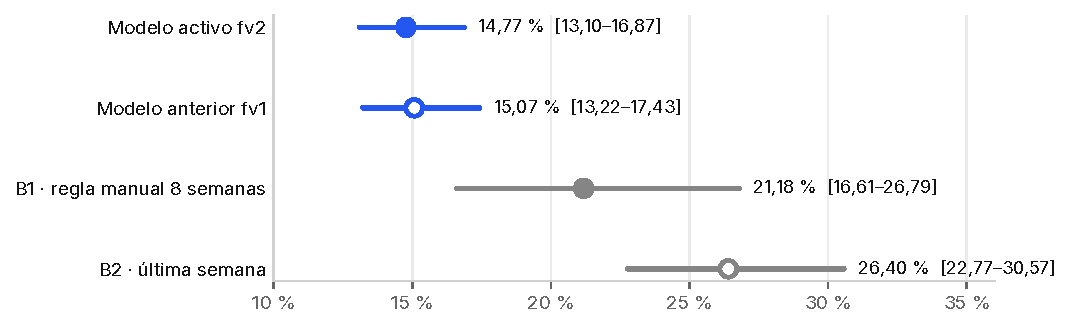
\includegraphics[width=\linewidth]{wape_modelos}
\gris{Diferencia con la regla manual: IC95 de \DifActBunoIC{} puntos (bootstrap de bloques de 7 días). La prueba se
consultó al elegir fv2 frente a fv1: es informativa; la selección usó la validación y los años congelados, y pedimos a
Extreme un periodo de 2026 como prueba limpia. El 13,94 y el 13,62~\% del informe (experimentos 11 y 12) son otra
métrica: a 7 días y sobre todo 2025.}
\end{tarjeta}
\end{column}
\begin{column}{0.37\linewidth}
\begin{tarjeta}
\titulotarjeta{Robusto}
\begin{tabularx}{\linewidth}{@{}Xrr@{}}
& \textcolor{rol-modelo}{Modelo} & \gris{B1} \\
\midrule
SILENCIO & \WAPERutaSilencio & \WAPERutaSilencioBuno \\
CRA 54 & \WAPERutaCra & \WAPERutaCraBuno \\
CL 72 & \WAPERutaCl & \WAPERutaClBuno \\
Pico / valle & \WAPEPico{} / \WAPEValle & \\
Año 2024 & \RobDosmilveinticuatro & \RobDosmilveinticuatroBuno \\
Año 2025 & \RobDosmilveinticinco & \RobDosmilveinticincoBuno \\
2025 (fv3) & \RobCandDosmilveinticinco & \RobDosmilveinticincoBuno \\
\midrule
30 min & \HorTreinta & \HorTreintaBuno \\
60 min & \HorSesenta & \HorSesentaBuno \\
120 min & \HorCientoveinte & \HorCientoveinteBuno \\
\end{tabularx}
\vspace{2pt}\gris{WAPE en \%. Años completos con el modelo congelado al cierre del año anterior. HGB con pérdida
Poisson y \NVariables{} variables. fv3: candidato sin activar, con el calendario escolar.}
\end{tarjeta}
\end{column}
\end{columns}
\end{frame}

% 5 ---------------------------------------------------------------------------------------------------------------
\fte{\path{pronostico_corto_plazo/README.md}, \path{PROTOCOLO.md}, \path{resultados/prueba.json} y \path{panel/verificacion_extreme.json}}
\begin{frame}[t]
\cabecera{El pronóstico del enunciado}{Modelo predictivo · 20 \%}
\begin{columns}[T]
\begin{column}{0.5\linewidth}
\begin{tarjeta}
\titulotarjeta{WAPE en la prueba reservada (jul.–dic. de 2025)}
{\scriptsize\setlength{\tabcolsep}{4pt}
\begin{tabularx}{\linewidth}{@{}Xrrr@{}}
& 30 min & 60 min & 120 min \\
\midrule
Ruta & \textcolor{rol-modelo}{\CortoRutaTreinta} \gris{(\CortoRutaTreintaBase)} & \textcolor{rol-modelo}{\CortoRutaSesenta} \gris{(\CortoRutaSesentaBase)} & \textcolor{rol-modelo}{\CortoRutaCientoveinte} \gris{(\CortoRutaCientoveinteBase)} \\
Sentido & \textcolor{rol-modelo}{\CortoSentidoTreinta} \gris{(\CortoSentidoTreintaBase)} & \textcolor{rol-modelo}{\CortoSentidoSesenta} \gris{(\CortoSentidoSesentaBase)} & \textcolor{rol-modelo}{\CortoSentidoCientoveinte} \gris{(\CortoSentidoCientoveinteBase)} \\
Segmento & \textcolor{rol-modelo}{\CortoSegmentoTreinta} \gris{(\CortoSegmentoTreintaBase)} & \textcolor{rol-modelo}{\CortoSegmentoSesenta} \gris{(\CortoSegmentoSesentaBase)} & \textcolor{rol-modelo}{\CortoSegmentoCientoveinte} \gris{(\CortoSegmentoCientoveinteBase)} \\
\end{tabularx}}
\vspace{2pt}\gris{En \%: \textcolor{rol-modelo}{modelo} y, entre paréntesis, el promedio por día y hora, la línea base del
enunciado. Cada media hora, de 04:00 a 21:00, se pronostican las subidas de los siguientes 30, 60 y 120 minutos con
lo observado hasta ese instante (LightGBM con pérdida Poisson). Por ruta a 60 min, la diferencia tiene un IC95 de
\CortoDifIC{} puntos y la banda P10--P90 cubre el \CortoCobertura~\%.}
\end{tarjeta}
\end{column}
\begin{column}{0.47\linewidth}
\begin{tarjeta}
\scriptsize\titulotarjeta{Validación y prueba separadas}
Protocolo confirmado en git antes de validar: todo se eligió con \textbf{ene.--jun. de 2025} y la prueba de
\textbf{jul.--dic.} se calculó una sola vez.
\end{tarjeta}
\begin{tarjeta}
\scriptsize\titulotarjeta{Lo espacial, con tres años}
\CortoSubidas{} subidas asignadas a los 386 segmentos con la regla de Extreme (antes, 37 días). El modelo gana al
promedio en \CortoSegGana{} de \CortoSegTotal{} segmentos.
\end{tarjeta}
\begin{tarjeta}
\scriptsize\titulotarjeta{Lo que falta}
Llevarlo a la API, que hoy pronostica por hora de salida. El sentido es una aproximación y 2025 ya se conocía, con
otro objetivo.
\end{tarjeta}
\end{column}
\end{columns}
\end{frame}

% 6 ---------------------------------------------------------------------------------------------------------------
\fte{\path{api_frecuencias/docs/evidencias/modelo/} (con \path{segmentos_modelo.json}), \path{.../monitoreo/compuerta_ejemplo.json}, \path{.../monitoreo/onnx_paridad.json}, \path{.../tablero/}\pantalla{dash_monitoreo.png}{operacion_monitoreo_1366x768.png}}
\begin{frame}[t]
\cabecera{Incertidumbre y ciclo de vida}{Modelo predictivo · 20 \%}
\begin{columns}[T]
\begin{column}{0.47\linewidth}
\begin{tarjeta}
\begin{minipage}[t]{0.47\linewidth}\cifraazul{\CobModelo~\%}{cobertura de la banda P10--P90 (objetivo 80~\%)}\end{minipage}\hfill
\begin{minipage}[t]{0.47\linewidth}\cifra{\CobVdos~\%}{con la calibración conformal versionada (ajustada solo con la validación)}\end{minipage}
\end{tarjeta}
\begin{tarjeta}
\scriptsize\titulotarjeta{Por qué (§9.4)}
SHAP local por pronóstico (base × factores = pronóstico, error $<10^{-6}$) e importancia global por API.
\end{tarjeta}
\begin{tarjeta}
\scriptsize\titulotarjeta{Aprendizaje controlado (RF-018, RF-019)}
PSI y error móvil de 28 días → reentrenar → 14 días en sombra → compuerta de 4 criterios → activar con auditoría o
rechazar; reversión automática en 7 días. Ejemplo: candidato \GateWAPECand~\% frente a \GateWAPEAct~\% del activo:
\textbf{\GateDecision}. ONNX: \OnnxDifMax{} pasajeros de diferencia máxima y \OnnxMsFila{} ms por fila.
\end{tarjeta}
\end{column}
\begin{column}{0.5\linewidth}
\begin{tarjeta}[left=3pt,right=3pt,top=3pt,bottom=3pt]
\centering\begin{minipage}{0.86\linewidth}\captura{dash_monitoreo}{operacion_monitoreo_1366x768}\end{minipage}
\end{tarjeta}
{\scriptsize\gris{Tablero, pantalla Monitoreo: error, sesgo, cobertura y deriva del modelo activo, desde la API.}}
\par\vspace{2pt}
\begin{tarjeta}
\scriptsize\titulotarjeta{Por segmento y sentido (§3.1, §9.1)}
Un modelo propio reparte el pronóstico de la ruta. Prueba de feb.~2023: WAPE por segmento y hora de
\textbf{\SegWAPEact~\%} (reparto fijo: \SegWAPEbcero~\%); banda P10--P90 con \SegCobSegmento~\% de cobertura por
segmento. La tabla de Extreme solo trae subidas por segmento de ene.--feb.~2023: el pronóstico por segmento con
tres años es el de la lámina anterior.
\end{tarjeta}
\end{column}
\end{columns}
\end{frame}

% 7 ---------------------------------------------------------------------------------------------------------------
\fte{\path{api_frecuencias/docs/evidencias/optimizacion/sensibilidad.md}, \path{ejemplo_calculate_no_viable.json}, \path{.../tablero/}\pantalla{dash_recomendaciones.png}{recomendaciones_1366x768.png}}
\begin{frame}[t]
\cabecera{Recomendaciones viables}{Optimización y alertas · 20 \%}
\begin{columns}[T]
\begin{column}{0.44\linewidth}
\begin{tarjeta}
\raggedright
\titulotarjeta{Función objetivo de §10.2, en COP por hora}
{\small min α·costo + β·espera\\ \quad + γ·sobreocupación + δ·desviación}\par\vspace{3pt}
\scriptsize\gris{sujeto a headway mínimo gobernado y máximo efectivo (el menor entre el máximo y 2 × la espera máxima,
S12), capacidad efectiva ≥ P90 calibrado (nivel de servicio 0,90), vehículos del ciclo ≤ flota, y flota por
tipología. El plan del día usa el pronóstico horario del modelo activo. Elasticidad: estimada ≈~0,70 por observación
(informe, §4.2), sin validar en campo; el plan usa 0,5 por prudencia y el piloto la mide.}
\end{tarjeta}
\begin{tarjeta}
\raggedright
\begin{tabular}{@{}p{0.46\linewidth}p{0.46\linewidth}@{}}
\leavevmode{\fontsize{21}{23}\selectfont\textcolor{rol-modelo}{\FranjasMilpIgual{}/\FranjasTotal}} &
\leavevmode{\fontsize{21}{23}\selectfont\FranjasViables{}/\FranjasTotal} \\
\scriptsize\gris{franjas reales en que el MILP (PuLP/CBC) coincide con la enumeración exacta} &
\scriptsize\gris{viables; las otras salen \emph{no viables} con motivo y mejor aproximación} \\
\end{tabular}
\end{tarjeta}
\end{column}
\begin{column}{0.53\linewidth}
\begin{tarjeta}[left=3pt,right=3pt,top=3pt,bottom=3pt]
\centering\begin{minipage}{0.76\linewidth}\captura{dash_recomendaciones}{recomendaciones_1366x768}\end{minipage}
\end{tarjeta}
{\scriptsize\gris{Tablero, pantalla Recomendaciones: lo recomendado frente a lo programado, con su explicación;
además, fórmulas de §10.3, tipologías T1--T4, escenarios y 23 variaciones de sensibilidad (RF-008).}}
\par\vspace{2pt}
\begin{tarjeta}
\scriptsize\titulotarjeta{Ocupación por segmento (§10.1)}
Carga a bordo de las subidas y bajadas de cada viaje (correlación \OcupCorrelacion{} con el dispositivo). Con la
ocupación actual, el plan pone un piso de salidas en los ciclos intradía de cada hora.
\end{tarjeta}
\end{column}
\end{columns}
\end{frame}

% 8 ---------------------------------------------------------------------------------------------------------------
\fte{\path{api_frecuencias/docs/evidencias/alertas/}: \path{backtest_alertas.md}, \path{backtest_alertas_pronostico.md}, \path{identificacion_viajes.md}; \path{.../tablero/}\pantalla{dash_alertas.png}{alertas_detalle_1366x768.png}}
\begin{frame}[t]
\cabecera{Alertas que se pueden creer}{Optimización y alertas · 20 \%}
\begin{columns}[T]
\begin{column}{0.47\linewidth}
\begin{tarjeta}
\titulotarjeta{Alertas observadas por ruta y día (\DiasRuta{} días-ruta fuera de muestra)}
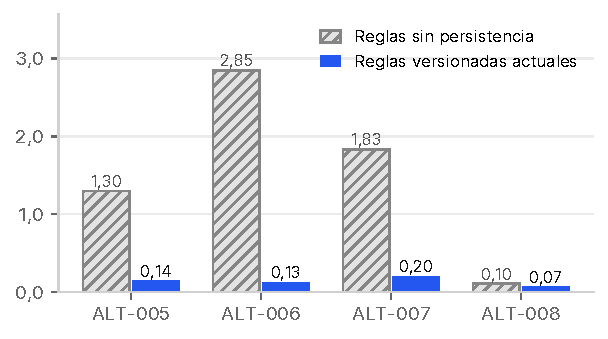
\includegraphics[width=0.86\linewidth]{alertas_por_ruta_dia}\par
\scriptsize\gris{Persistencia de 2 horas y una alerta por episodio: de \AlertasAntes{} a \AlertasAhora{} (ALT-005 a
ALT-009). Lift (precisión / tasa base): ALT-005 \LiftCinco, ALT-006 \LiftSeis, ALT-007 \LiftSiete, ALT-008 \LiftOcho{}
(subidas, bajadas y viajes). Con ALT-002 observada y las rupturas son \AlertasObsTodas; con las de pronóstico del ciclo
diario (\AlertasPronostico, una por franja), \AlertasTotal{} en total. ALT-003 exige una probabilidad mínima de superar
la capacidad efectiva, elegida sin fuga (migración 0014, propuesta). Si un episodio se agrava, la alerta escala y queda
en la bitácora.}
\end{tarjeta}
\end{column}
\begin{column}{0.5\linewidth}
\begin{tarjeta}[left=3pt,right=3pt,top=3pt,bottom=3pt]
\captura{dash_alertas}{alertas_detalle_1366x768}
\end{tarjeta}
\begin{tarjeta}
\scriptsize\gris{Cada alerta (§5.3) trae real, esperado y umbral en las mismas unidades, tendencia, puntaje con su método,
variables influyentes (SHAP), recomendación, ubicación \texttt{geography} con GiST y bitácora de estados (RF-011), y
dice qué campos de identificación le aplican: ALT-006 y ALT-009 llevan el viaje, el vehículo y el seudónimo del
conductor.}
\end{tarjeta}
\end{column}
\end{columns}
\end{frame}

% 9 ---------------------------------------------------------------------------------------------------------------
\fte{\path{api_frecuencias/docs/evidencias/replica/}: \path{replica_roles.txt}, \path{replica_llegada.txt}, \path{explain_incremental.txt}; intentos: \FuenteIntentos; \path{.../cola/replicas_por_ruta.json}, \path{.../pruebas/k6_segmentos_consultas.json}, \path{.../pruebas/k6_segmentos.txt}}
\begin{frame}[t]
\cabecera{Se conecta sin interferir}{Integración y rendimiento · 15 \%}
\begin{columns}[T]
\begin{column}{0.5\linewidth}
\begin{tarjeta}
\titulotarjeta{Probado en una réplica con los scripts y el trigger de Extreme}
\begin{itemize}
\item \textbf{0 escrituras indebidas en \NIntentosTotal{} intentos}: \NIntentosLector{} de \texttt{lector\_ia} (16 tipos
de sentencia) y \NIntentosEscritor{} de \texttt{escritor\_ia} sobre 14 tablas de Extreme (42501);
\item 584 eventos reales pasan por el trigger y la API entrega \textbf{exactamente 1 franja nueva}; sin datos
nuevos, lee 0;
\item \texttt{EXPLAIN (ANALYZE, BUFFERS)}: la lectura diaria baja de 122 ms a 0,01 ms con el índice que proponemos
(lo aplica su DBA, nunca la aplicación);
\item \textbf{partición por ruta} (RNF-005): dos réplicas procesan rutas distintas a la vez, nunca la misma, y dan
las mismas salidas que sin partir.
\end{itemize}
\end{tarjeta}
\end{column}
\begin{column}{0.47\linewidth}
\begin{tarjeta}
\titulotarjeta{Consultas paginadas con k6: p95 por recurso}
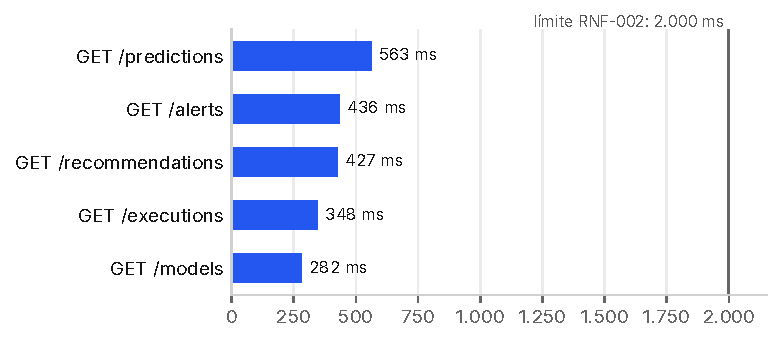
\includegraphics[width=\linewidth]{k6_p95}
\gris{\Kpeticiones{} peticiones, \Kerrores~\% de errores; durante una ingesta, p95 de \Kingesta{} ms. Ingesta de
\IngestaFilas{} filas en \IngestaSegundos{} s (RNF-003).}
\end{tarjeta}
\begin{tarjeta}
\scriptsize\titulotarjeta{Capa de segmentos (RNF-002)}
\texttt{GET /segmentos/estadisticas} lee una agregación materializada: \textbf{\SegFrio{} ms} la primera petición y
p95 de \SegCarga{} ms con hasta \SegCargaUsuarios{} usuarios durante un refresco.
\end{tarjeta}
\end{column}
\end{columns}
\end{frame}

% 10 ---------------------------------------------------------------------------------------------------------------
\fte{\FuentePruebas; \FuenteCobertura; \path{api_frecuencias/docs/evidencias/sonarqube/measures.json}; \path{api_frecuencias/ci/github_actions_entrega.yml}}
\begin{frame}[t]
\cabecera{Ingeniería que se puede auditar}{Ingeniería de software · 15 \%}
\begin{columns}[T]
\begin{column}{0.47\linewidth}
\begin{tarjeta}
\titulotarjeta{\Ntotal{} pruebas automáticas en seis niveles}
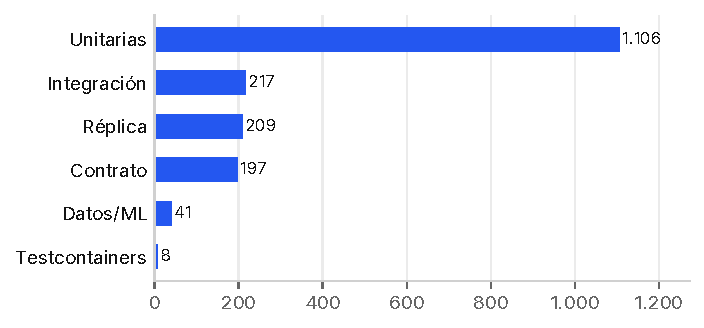
\includegraphics[width=\linewidth]{pruebas_por_nivel}
\gris{\Npasan{} aprobadas, \Nfallan{} fallidas y \Nomitidas{} omitidas a propósito, en la \CorridaPruebas.}
\end{tarjeta}
\end{column}
\begin{column}{0.5\linewidth}
\begin{tarjeta}
\begin{columns}[T]
\begin{column}{0.48\linewidth}\cifraazul{\Cobertura~\%}{cobertura de líneas de \texttt{app/}}\end{column}
\begin{column}{0.48\linewidth}\cifra{\NOperacionesVuno}{operaciones REST en \texttt{/api/v1}, con OpenAPI 3 y roles}\end{column}
\end{columns}
\end{tarjeta}
\begin{tarjeta}
\begin{itemize}
\item CI (GitHub Actions; Python 3.11 y 3.13): ruff, bandit, Alembic de ida y vuelta, pytest con cobertura mínima de
85~\%, Testcontainers y deriva del OpenAPI; \EstadoCICorto;
\item \SonarResumen;
\item Docker Compose: API, PostgreSQL + PostGIS, migración y trazas;
\item logs JSON, \texttt{/metrics} y trazas OpenTelemetry.
\end{itemize}
\end{tarjeta}
\end{column}
\end{columns}
\end{frame}

% 11 --------------------------------------------------------------------------------------------------------------
\fte{\path{api_frecuencias/docs/evidencias/despliegue/demo_ciclo_api.txt} (\path{scripts/demo_ciclo_api.py} contra la API en Docker)}
\begin{frame}[t]
\cabecera{Demostración del ciclo de §14.2}{Presentación y adopción · 10 \%}
\vspace{4pt}
\begin{tikzpicture}[paso/.style={draw=rol-linea, fill=rol-superficie, rounded corners=8pt, text width=3.75cm,
  minimum height=2.15cm, align=left, inner sep=5pt, font=\scriptsize},
  num/.style={circle, fill=rol-modelo, text=rol-tinta-inversa, font=\scriptsize\intermedia, inner sep=1.6pt},
  fl/.style={-{Stealth[length=2mm]}, draw=rol-tinta-3, line width=0.7pt}]
\node[paso] (a) at (0,0) {\textbf{Llega información nueva}\\ tras la carga inicial (\DemoFilasInicial{} filas), el
día \DemoMarcaDespues{} aparece en la fuente, después de la marca de agua};
\node[paso, right=4mm of a] (b) {\textbf{Lectura incremental}\\ lee solo esas \DemoFilasNuevas{} filas (marca
\DemoMarcaAntes{} → \DemoMarcaDespues); repetir sin datos nuevos lee \DemoFilasRepeticion{} y no duplica};
\node[paso, right=4mm of b] (c) {\textbf{Evaluación del error}\\ WAPE del activo sobre lo recién llegado:
\DemoWapeNuevo~\%; el monitoreo registra error móvil, cobertura y PSI};
\node[paso, below=5mm of c] (d) {\textbf{Modelo candidato}\\ \texttt{POST /models/train}: job asíncrono con progreso;
\DemoCandidato{} entrenado en \DemoEntrenoSeg{} s};
\node[paso, left=4mm of d] (e) {\textbf{Comparación con el activo}\\ misma validación temporal (\DemoVentana): WAPE
\DemoWapeCand~\% del candidato frente a \DemoWapeAct~\% del activo};
\node[paso, left=4mm of e] (f) {\textbf{Decisión}\\ \DemoDecision{} (409): el activo se conserva y la decisión queda
en el registro de modelos, auditada y reversible};
\foreach \n/\k in {a/1,b/2,c/3,d/4,e/5,f/6} \node[num] at (\n.north west) {\k};
\draw[fl] (a) -- (b); \draw[fl] (b) -- (c); \draw[fl] (c) -- (d); \draw[fl] (d) -- (e); \draw[fl] (e) -- (f);
\end{tikzpicture}
\vspace{3pt}

{\scriptsize\gris{Ciclo completo en \DemoTotalSeg{} s con \texttt{scripts/demo\_ciclo\_api.py} contra la API en Docker;
cada paso deja su ejecución en \texttt{execution\_log} y su decisión en \texttt{model\_registry}.}}
\end{frame}

% 12 --------------------------------------------------------------------------------------------------------------
\fte{\path{api_frecuencias/docs/evidencias/respuesta/}: \RespuestaFuente{} y \RespuestaEjemploFuente; alertas: \path{.../alertas/backtest_alertas.md} y \path{backtest_alertas_pronostico.md}; detalle: \path{documentos/respuesta_pregunta_reto.md}}
\begin{frame}[t]
\cabecera{La respuesta a la pregunta}{§20 · \RespuestaTipoDia{} \RespuestaFecha}
\begin{tarjeta}
\scriptsize\setlength{\tabcolsep}{3pt}
\begin{tabularx}{\linewidth}{@{}l>{\raggedright\arraybackslash}p{1.6cm}>{\raggedright\arraybackslash}p{2.5cm}>{\raggedright\arraybackslash}p{1.3cm}>{\raggedright\arraybackslash}p{2.9cm}>{\raggedright\arraybackslash}p{1.5cm}>{\raggedright\arraybackslash}X@{}}
\toprule
Ruta & Salidas al día: plan / hoy & Cada cuánto (min): pico mañana / valle / pico tarde & Horas no viables &
Pasajeros esperados (P10--P90) & Buses en ruta: pico / flota & Recaudo / costo (M COP) \\
\midrule
\RespuestaFilas
\bottomrule
\end{tabularx}
\end{tarjeta}
\begin{tarjeta}
\scriptsize\textbf{Atención inmediata.} Con los umbrales vigentes se esperan \AlertasTotal{} alertas por ruta y día:
\AlertasObsTodas{} observadas y \AlertasPronostico{} de pronóstico (ALT-001 \AlertasPronUno, ALT-002 \AlertasPronDos,
ALT-003 \AlertasPronTres). La respuesta lista las abiertas ahora, críticas primero, y aparte las detectadas en la
fecha consultada. Por ejemplo, \RespuestaEjemplo
\end{tarjeta}
{\fontsize{6.5}{8}\selectfont\gris{\texttt{GET /api/v1/respuesta}. Cada cuánto = minutos operados / salidas de la
franja (pico mañana 6--8~h, valle 9--16~h, pico tarde 17--19~h), como en \texttt{respuesta\_pregunta\_reto.md}; en
gris, lo programado hoy. Una hora no viable programa la mejor aproximación ejecutable, con su motivo. Pasajeros del
modelo \RespuestaModelo; recaudo con tarifa pública de referencia (§19).}}
\end{frame}

% 13 --------------------------------------------------------------------------------------------------------------
\fte{\path{Informe_tecnico_Sobusa.pdf}, §4 (tabla 8 de escenarios y figura del plan que reasigna; sus datos están en el repositorio del proyecto, no en esta entrega)}
\begin{frame}[t]
\cabecera{Qué gana Sobusa}{Valor para la operación}
\begin{columns}[T]
\begin{column}{0.52\linewidth}
\begin{tarjeta}[left=3pt,right=3pt,top=3pt,bottom=3pt]
\IfFileExists{figuras/plan_reasigna.pdf}{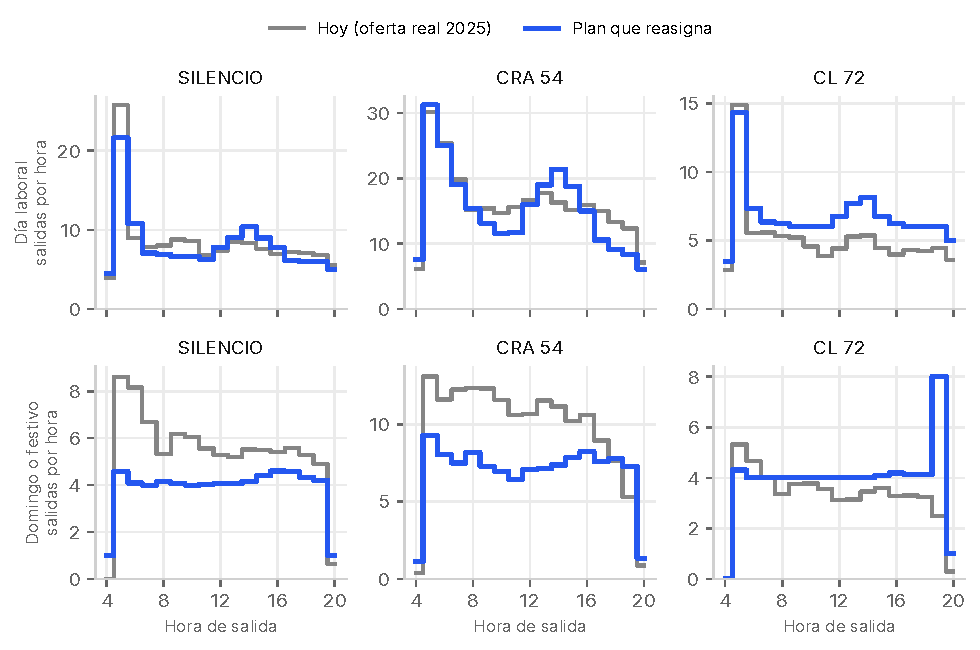
\includegraphics[width=\linewidth]{plan_reasigna}}%
{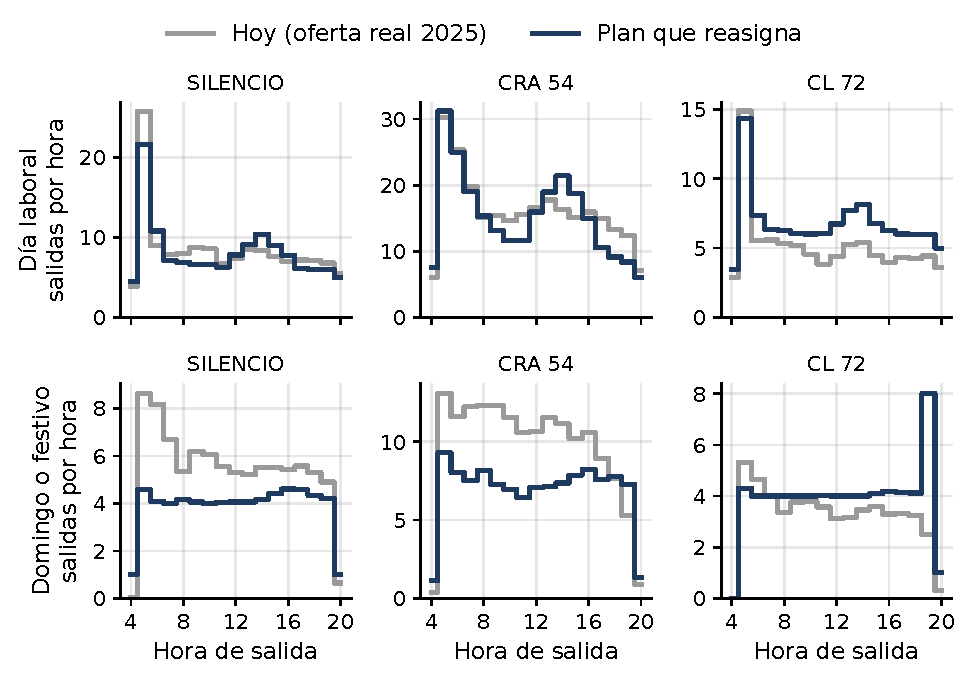
\includegraphics[width=\linewidth]{fig_plan_reasigna}}
\end{tarjeta}
{\scriptsize\gris{Salidas por hora, promedio por día de 2025: hoy (gris) y el plan que reasigna (azul); misma figura
del informe, §4. Cifras del informe académico: todo 2025 con el pronóstico a 7 días del experimento 12; el producto
calcula el plan con el modelo activo.}}
\end{column}
\begin{column}{0.45\linewidth}
\begin{tarjeta}
\begin{columns}[T]
\begin{column}{0.48\linewidth}\cifraazul{451}{salidas al día frente a 460}\end{column}
\begin{column}{0.48\linewidth}\cifraazul{4,30}{minutos de espera frente a 4,43}\end{column}
\end{columns}\vspace{4pt}
\begin{columns}[T]
\begin{column}{0.48\linewidth}\cifraazul{267}{pasajeros al día sobre la capacidad, frente a 317}\end{column}
\begin{column}{0.48\linewidth}\cifra{+501}{M COP al año en operación}\end{column}
\end{columns}
\end{tarjeta}
\begin{tarjeta}
\gris{Saldo anual entre \textbf{−2.825 M COP} (contando solo los pasajeros perdidos) y \textbf{+1.600 M COP}
(contando también los ganados). El plan que \textcolor{rol-recorta}{recorta} deja más caja (+1.939 M COP) pero pierde
1.512 pasajeros netos al día y sube a 530 los pasajeros sobre la capacidad. El piloto mide cuál contabilidad vale.}
\end{tarjeta}
\end{column}
\end{columns}
\end{frame}

% 14 --------------------------------------------------------------------------------------------------------------
\fte{\path{PLAN_EVOLUCION.md} (§1.1 calendario y criterio, §3.1 costos, §4 riesgos); \path{Informe_tecnico_Sobusa.pdf}, §4 (piloto); sensibilidad de β: \path{api_frecuencias/docs/evidencias/optimizacion/sensibilidad.md}}
\begin{frame}[t]
\cabecera{Plan de implementación}{Presentación y adopción · 10 \%}
\begin{tikzpicture}[fase/.style={draw=rol-linea, fill=rol-superficie, rounded corners=8pt, text width=4.0cm,
  minimum height=2.5cm, align=left, inner sep=5pt, font=\scriptsize},
  faseazul/.style={fase, draw=rol-modelo, fill=rol-acento-suave}]
\node[fase] (s1) at (0,0) {\textbf{Semanas \PlanSemanasConexion{} · Conexión}\\ respuestas a los hallazgos;
réplica de lectura y usuarios \texttt{lector\_ia} y \texttt{escritor\_ia}; el DBA revisa el EXPLAIN y decide el
índice; migraciones; parámetros operativos reales.\\[2pt]
\gris{Sigue si: mismos conteos que la exportación en tres semanas de control.}};
\node[fase, right=4mm of s1] (s2) {\textbf{Semanas \PlanSemanasSombra{} · Modo sombra}\\ el ciclo diario corre y
nadie despacha con él; se mide el error a 30/60/120 min, la cobertura y las alertas descartadas.\\[2pt]
\gris{Sigue si: \PlanCriterioSombra.}};
\node[faseazul, right=4mm of s2] (s3) {\textbf{Semanas \PlanSemanasPiloto{} · Piloto}\\ ocho semanas en CRA~54 y
CL~72 con días sorteados para medir la elasticidad (probabilidad 0,92 y 0,89); arriesga 22.904 pasajeros, el
0,30~\% del año de CRA~54.\\[2pt] \gris{El despachador decide; el sistema recomienda.}};
\end{tikzpicture}
\vspace{4pt}
\begin{columns}[T]
\begin{column}{0.48\linewidth}
\begin{tarjeta}
\titulotarjeta{Costos de infraestructura (USD al mes, orden de magnitud)}
En la plataforma de Extreme: \textbf{\PlanCostoTotalA} (cómputo \PlanCostoComputo; base de resultados y réplica, las
de Extreme). En una nube propia administrada: \PlanCostoTotalB. Software libre, sin licencias; lo que más pesa son las
personas (el analista en sombra y piloto).
\end{tarjeta}
\end{column}
\begin{column}{0.48\linewidth}
\begin{tarjeta}
\titulotarjeta{Riesgos y mitigación}
elasticidad estimada ≈~0,70, sin validar en campo → el plan usa 0,5 y el piloto la mide · fatiga de alertas → persistencia,
episodios y escalamiento · parámetros de §19 sin confirmar → umbrales, flota y ciclo versionados · deriva → sombra,
compuerta y reversión.
\end{tarjeta}
\end{column}
\end{columns}
\end{frame}

% 15 --------------------------------------------------------------------------------------------------------------
\fte{\path{api_frecuencias/docs/hallazgos_extreme.md}; \path{README.md}; \path{PLAN_EVOLUCION.md}; E01 y E02}
\begin{frame}[t]
\vspace{10pt}
{\fontsize{26}{30}\selectfont La decisión que pedimos}\par\vspace{10pt}
\begin{columns}[T]
\begin{column}{0.31\linewidth}
\begin{tarjeta}[height=3.6cm]
\cifraazul{1}{}
\textbf{Una réplica de lectura} y los dos usuarios, para correr el ciclo diario contra los datos reales en modo
sombra.
\end{tarjeta}
\end{column}
\begin{column}{0.31\linewidth}
\begin{tarjeta}[height=3.6cm]
\cifraazul{2}{}
\textbf{Respuestas a \PlanHallazgosUrgentes} y los parámetros de §19: capacidad, ciclo, flota y límites de headway
oficiales.
\end{tarjeta}
\end{column}
\begin{column}{0.31\linewidth}
\begin{tarjeta}[height=3.6cm]
\cifraazul{3}{}
\textbf{Aprobar el piloto de ocho semanas} en CRA~54 y CL~72, con el despachador al mando.
\end{tarjeta}
\end{column}
\end{columns}
\vspace{10pt}
{\small\gris{Todo es reproducible: \texttt{docker compose up} levanta la API con su PostgreSQL; las cifras de estos
documentos salen de las evidencias con \texttt{python documentos/compilar.py}.}}\par\vspace{6pt}
{\small Gracias. \gris{Abrahan Basto Martínez · Rubén Esguerra Fernández · Paula Gómez}}
\end{frame}

\end{document}
